\section{Bias Variance Decomposition}

  Determination of the predictive distribution $p(y\,|\,x)$ given data $\mathcal{D}$ is the goal of statistical inference, as we have seen. That is, posterior $p(y\,|\,x, \mathcal{D})$ tells us the distribution of $y$ if we have a new data point $x$. But after this inference step, we must look now at the \textbf{decision step}: we must determine a function $h(x)$ that deterministically predicts a value $y$, without predictions. That is, we must have some algorithm to make a decision.

  Let us zoom out for a better overview. Let $\mathcal{D}$ be our training data of $N$ points. We can assume that each point $(x_i, y_i) \in \mathcal{D}$ was \textit{generated} independently by a joint distribution $p(x, y)$. If we were to get another data point, we would just generate one from the density $p(x, y)$. Usually, we have fixed input data $x$ and knew that the output $y$ given $x$ would be $p(y\,|\,x)$. But if we loosen our constraint on $x$, we would get
  \begin{equation}
    p(x, y) = p(y\,|\,x) p(x)
  \end{equation}

  which states that each data point in $\mathcal{D}$ is gotten by generating a value of $x$ with probability $p(x)$, and then generating a $y$ given this $x$. Let us also denote $\mathcal{A}$ as our machine learning algorithm, which we can interpret as a function that takes in data $\mathcal{D}$ and outputs the hypothesis function $h_\mathcal{D}$.
  \begin{equation}
    \mathcal{A} (\mathcal{D}) = h_\mathcal{D}
  \end{equation}

  Then, given that the next new data point $(x, y)$ is generated, we can set our \textbf{test error}, or \textbf{loss/cost function}, of $h_\mathcal{D}$ to be
  \begin{equation}
    L\big(h_\mathcal{D}, (x, y) \big) = \big[ h_\mathcal{D} (x) - y \big]^2
  \end{equation}

  This loss function basically calculates the inaccuracy of whatever hypothesis function $h_\mathcal{D}$ we have on the data $(x, y)$, which in this case is the square of the residual. There can be other types of loss functions, but we will consider the squares loss function for now. Given $h_\mathcal{D}$, we can also calculate the expected test error by conditioning over all $x, y$ drawn from $P$.
  \begin{equation}
    \text{Expected Test Error given } h_\mathcal{D} \implies \mathbb{E}_{x, y, \sim P} \big[ (h_\mathcal{D} (x) - y)^2 \big] = \int_x \int_y (h_\mathcal{D} (x) - y)^2 \, p(x, y)\; dy \, dx
  \end{equation}

  However, note that we can treat the $N$ data points $\mathcal{D}$ also as a random variable coming from the joint distribution of $N$ $P$'s. Therefore, we can take each possible dataset $\mathcal{D}$, calculate $h_\mathcal{D} = \mathcal{A}(\mathcal{D})$ with our algorithm, and average them out to get the expected hypothesis function $\overline{h}$. We can interpret $\overline{h}$ as the "ideal regressor" that we are trying to build, but with limited data $\mathcal{D}$, we can only build $h_\mathcal{D}$ that deviates from $\overline{h}$.
  \begin{equation}
    \overline{h} = \mathbb{E}_{\mathcal{D} \sim P^N} \big[ \mathcal{A}(\mathcal{D}) \big] = \int_\mathcal{D} h_\mathcal{D} P(\mathcal{D})\; d\mathcal{D}
  \end{equation}

  So, we can compute the expected error of the \textit{entire algorithm} $\mathcal{A}$ by marginalizing over all $x, y$ given $h_\mathcal{D}$ and marginalizing over all $\mathcal{D}$. Remember that $D \sim P^N$ is our training data of $N$ points, and $(x, y) \sim P$ is our $(n+1)$th data point. Therefore, the expected test error of our \textit{algorithm} for the $(n+1)$th data point is
  \begin{equation}
    \mathbb{E}_{(x, y) \sim P, \mathcal{D} \sim P^N} \big( [ h_\mathcal{D} (x) - y]^2 \big) = \int_\mathcal{D} \int_x \int_y [ h_\mathcal{D} (x) - y]^2\, p(x, y) \, p(\mathcal{D})\; dy\,dx\,d\mathcal{D}
  \end{equation}

  The integral above looks quite intimidating, so let us decompose it. We just have do use a trick where we subtract and add the same term $\overline{h}(x)$.
  \begin{align*}
    \mathbb{E}_{(x, y), \mathcal{D}} \big( [ h_\mathcal{D} (x) - y]^2 \big) & = \mathbb{E}_{(x, y), \mathcal{D}} \big( [ (h_\mathcal{D} (x) - \overline{h}(x)) + (\overline{h}(x) - y)]^2 \big) \\
    & = \mathbb{E}_{(x, y), \mathcal{D}} \big( [h_\mathcal{D} (x) - \overline{h} (x)]^2 \big) + 
    \mathbb{E}_{(x, y), \mathcal{D}} \big( [\overline{h} (x) - y]^2 \big) \\
    & \;\;\;\;\;\;\;\;\; + 2 \mathbb{E}_{(x, y), \mathcal{D}} \big([h_\mathcal{D} (x) - \overline{h} (x)]\,[\overline{h} (x) - y] \big)
  \end{align*}

  But I claim that the last term vanishes. It is easy to see why because
  \begin{align*}
    \mathbb{E}_{(x, y), \mathcal{D}} \left[\left(h_{\mathcal{D}}(x) - \bar{h}(x)\right) \left(\bar{h}(x) - y\right)\right] 
    &= \mathbb{E}_{(x, y)} \left[E_{\mathcal{D}} \left[ h_{\mathcal{D}}(x) - \bar{h}(x)\right] \left(\bar{h}(x) - y\right) \right] \\
    &= \mathbb{E}_{(x, y)} \left[ \left( E_{\mathcal{D}} \left[ h_{\mathcal{D}}(x) \right] - \bar{h}(x) \right) \left(\bar{h}(x) - y \right)\right] \\
    &= \mathbb{E}_{(x, y)} \left[ \left(\bar{h}(x) - \bar{h}(x) \right) \left(\bar{h}(x) - y \right)\right] \\
    &= \mathbb{E}_{(x, y)} \left[ 0 \right] \\
    &= 0
  \end{align*}

  Therefore, we can see that the expected value of the error of an algorithm consists of two terms: the variance and the second term.
  \begin{equation}
    \mathbb{E}_{(x, y), \mathcal{\mathcal{D}}} \big( [ h_\mathcal{\mathcal{D}} (x) - y]^2 \big) = \mathbb{E}_{(x, y), \mathcal{\mathcal{D}}} \big( [h_\mathcal{\mathcal{D}} (x) - \overline{h} (x)]^2 \big) + 
    \mathbb{E}_{(x, y), \mathcal{\mathcal{D}}} \big( [\overline{h} (x) - y]^2 \big)
  \end{equation}

  The second term is the expected value of the average prediction minus the $y$-value of the new point. Now, we do the same trick: Let the expected value of $y$ given $x$ be $\overline{y}(x) = \mathbb{E}_{y\,|\,x} (y) = \int y\, p(y\,|\,x)\; dx$. This function $\overline{y}(x)$ is the ideal regressor predicting $y$ from $x$. Then, we have
  \begin{align*}
    \mathbb{E}_{x, y} \left[ \left(\bar{h}(x) - y \right)^{2}\right] &= \mathbb{E}_{x, y} \left[ \left(\bar{h}(x) -\bar y(x) )+(\bar y(x) - y \right)^{2}\right] \\
    &=\underbrace{\mathbb{E}_{x, y} \left[\left(\bar{y}(x) - y\right)^{2}\right]}_\mathrm{Noise} + \underbrace{\mathbb{E}_{x} \left[\left(\bar{h}(x) - \bar{y}(x)\right)^{2}\right]}_\mathrm{Bias^2} + 2 \mathrm{\;} \mathbb{E}_{x, y} \left[ \left(\bar{h}(x) - \bar{y}(x)\right)\left(\bar{y}(x) - y\right)\right]
  \end{align*}

  where the third term vanishes since
  \begin{align*}
    \mathbb{E}_{x, y} \left[\left(\bar{h}(x) - \bar{y}(x)\right)\left(\bar{y}(x) - y\right)\right] 
    &= \mathbb{E}_{x}\left[\mathbb{E}_{y \mid x} \left[\bar{y}(x) - y \right] \left(\bar{h}(x) - \bar{y}(x) \right) \right] \\
    &= \mathbb{E}_{x} \left[ \left( \bar{y}(x) - \mathbb{E}_{y \mid x} \left [ y \right]\right) \left(\bar{h}(x) - \bar{y}(x)\right)\right] \\
    &= \mathbb{E}_{x} \left[ \left( \bar{y}(x) - \bar{y}(x) \right) \left(\bar{h}(x) - \bar{y}(x)\right)\right] \\
    &= \mathbb{E}_{x} \left[ 0 \right] \\
    &= 0
  \end{align*}

  Therefore, the expected test error is precisely the sum of three things.
  \begin{equation*}
    \underbrace{\mathbb{E}_{x, y, \mathcal{D}} \left[\left(h_{\mathcal{D}}(x) - y\right)^{2}\right]}_\mathrm{Expected\;Test\;Error} = \underbrace{\mathbb{E}_{x, \mathcal{D}}\left[\left(h_{\mathcal{D}}(x) - \bar{h}(x)\right)^{2}\right]}_\mathrm{Variance} + \underbrace{\mathbb{E}_{x, y}\left[\left(\bar{y}(x) - y\right)^{2}\right]}_\mathrm{Noise} + \underbrace{\mathbb{E}_{x}\left[\left(\bar{h}(x) - \bar{y}(x)\right)^{2}\right]}_\mathrm{Bias^2}
  \end{equation*}

  To understand this term a bit deeper, recall the following: The function $\overline{y}(x)$, which outputs the expected value of $y$ given $x$, is the best possible regressor we can have. There are many different algorithms that we can choose to approximate $\overline{y}(x)$, so let us choose one learning algorithm $\mathcal{A}$. We just feed an arbitrary dataset $\mathcal{D}$ to $\mathcal{A}$, which outputs a hypothesis function $h_\mathcal{D}$. But this hypothesis function $h_\mathcal{D}$ is really just an approximation of the \textit{ideal} hypothesis function $\overline{h}$, which is the expectation of all hypotheses $h_\mathcal{D}$ (i.e. the hypothesis that $\mathcal{A}$ should generate when we feed it an infinite amount of data). So, by feeding $\mathcal{D}$ to $\mathcal{A}$, it generates a hypothesis function $h_\mathcal{D}(x)$, which approximates $\overline{h}(x)$, which hopefully is a good estimate of $\overline{y}(x)$.

  \begin{enumerate}
    \item The difference between a generated hypothesis function $h_\mathcal{D}(x)$ and the ideal hypothesis that it is trying to estimate according to learning algorithm $\mathcal{A}$ is represented by the variance. The variance term tells us how far each generated hypothesis $h_\mathcal{D}$ deviates from the ideal $\overline{h}$.
    
    \item The difference between the ideal hypothesis $\overline{h}(x)$ (according to algorithm $\mathcal{A}$) and the ideal regressor \textit{in general} $\overline{y}(x)$ is captured in the bias term. The bias term tells us how far our algorithm's ideal hypothesis deviates from the expectation of the conditional $p(y\,|\,x)$.
    
    \item The noise term represents the difference between the true value of $y$ and the best possible regressor $\overline{y}(x)$. But since the best we can do is find the expectation of the conditional $p(y\,|\,x)$, the deviation of the true values $y$ from the mean $\overline{y}$ is simply the noise. For example, if we have $p(y\,|\,x) = \mathcal{N} \big( y\,|\, w^T\phi(x), \epsilon \big)$, then the noise would simply be $\epsilon$. If the variance of $\epsilon$ is large, the noise would be large. Therefore, the same ideal regressor function $\overline{y}(x)$ would perform worse with a higher noise.
  \end{enumerate}

  If we are comparing this to the throwing-darts analogy, we can imagine the ideal function $\overline{y}(x)$ to be the bull's eye that we must hit. The different algorithms $\mathcal{A}$ represent different players throwing the darts. When one algorithm (player) is chosen, their vision can be skewed (perhaps their glasses is off), leading them to think that the target $\overline{h}(x)$ is somewhere else. If their target is far away from the bull's eye (i.e. $[\overline{h}(x) - \overline{y}(x)]^2$ is high), then their bias is high. Their skills in darts may just be bad, so even if their vision is good and they have a good sense of where to hit (low bias), for each time they throw the dart (i.e. each time the regressor function $h_\mathcal{D}$ is generated from data), it may be very off from their ideal target $\overline{h}(x)$.

  Therefore, if you are a data scientist and you find that your regression function is not accurate enough, it is your job to find out whether your bias is too high, your variance is too high, or whether there is too much noise, and fix the proper component. Generally, we would try to minimize this cost function, visualized below.

  \begin{figure}[H]
    \centering
    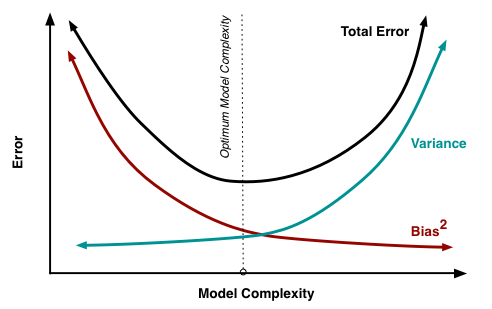
\includegraphics[width=0.5\textwidth]{img/biasvariance.png}
    \caption{Visualization of the bias-variance tradeoff showing how model complexity affects error components}
  \end{figure}

